\subsection{28 августа. Д.р. Чиринкол}

\textit{Метеоусловия: утром, днём, вечером переменная облачность, кратковременные дожди}

\begin{figure}[h!]
	\centering
	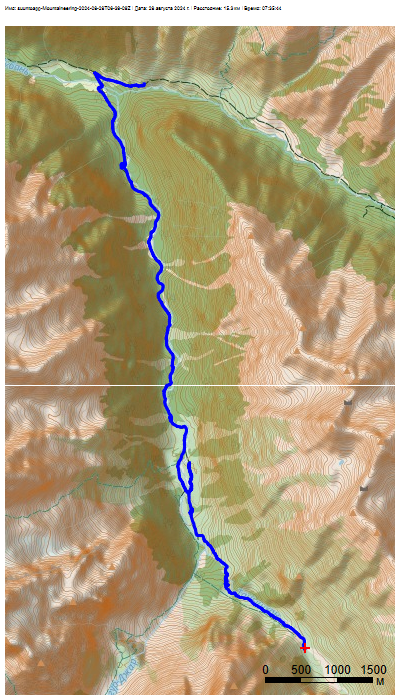
\includegraphics[angle=0, width=0.7\linewidth]{../pics/mini_maps/28}
	\label{fig:mini_28}
\end{figure}

\textbf{Чиринкол} (карач.-балк. <<Чирик-къол>>)~--- <<Гнилое ущелье>>.

Утром проснулись в 7:30. Ещё раз опросили двух собиравшихся сойти участников, Диму Сингалевича и Машу~--- они своего решения не поменяли. Вдобавок, к большой неожиданности для руководителя, о своём желании сойти с машрута, не беря пер. Хотютау, заявил Илья Шалфеев: он переживал из-за возможности задержаться при прохождении перевала и не вернуться в Москву строго ко времени. Предположительно, его не в последнюю очередь сильно подкосил выматывающий ночной спуск с Перемётного.

Для руководителя и замруководителя эта новость была сильным ударом. Да и в целом состояние группы в то утро было подавленным, --- хотя погода, напротив, стояла великолепная.
\begin{figure}[h!]
	\centering
	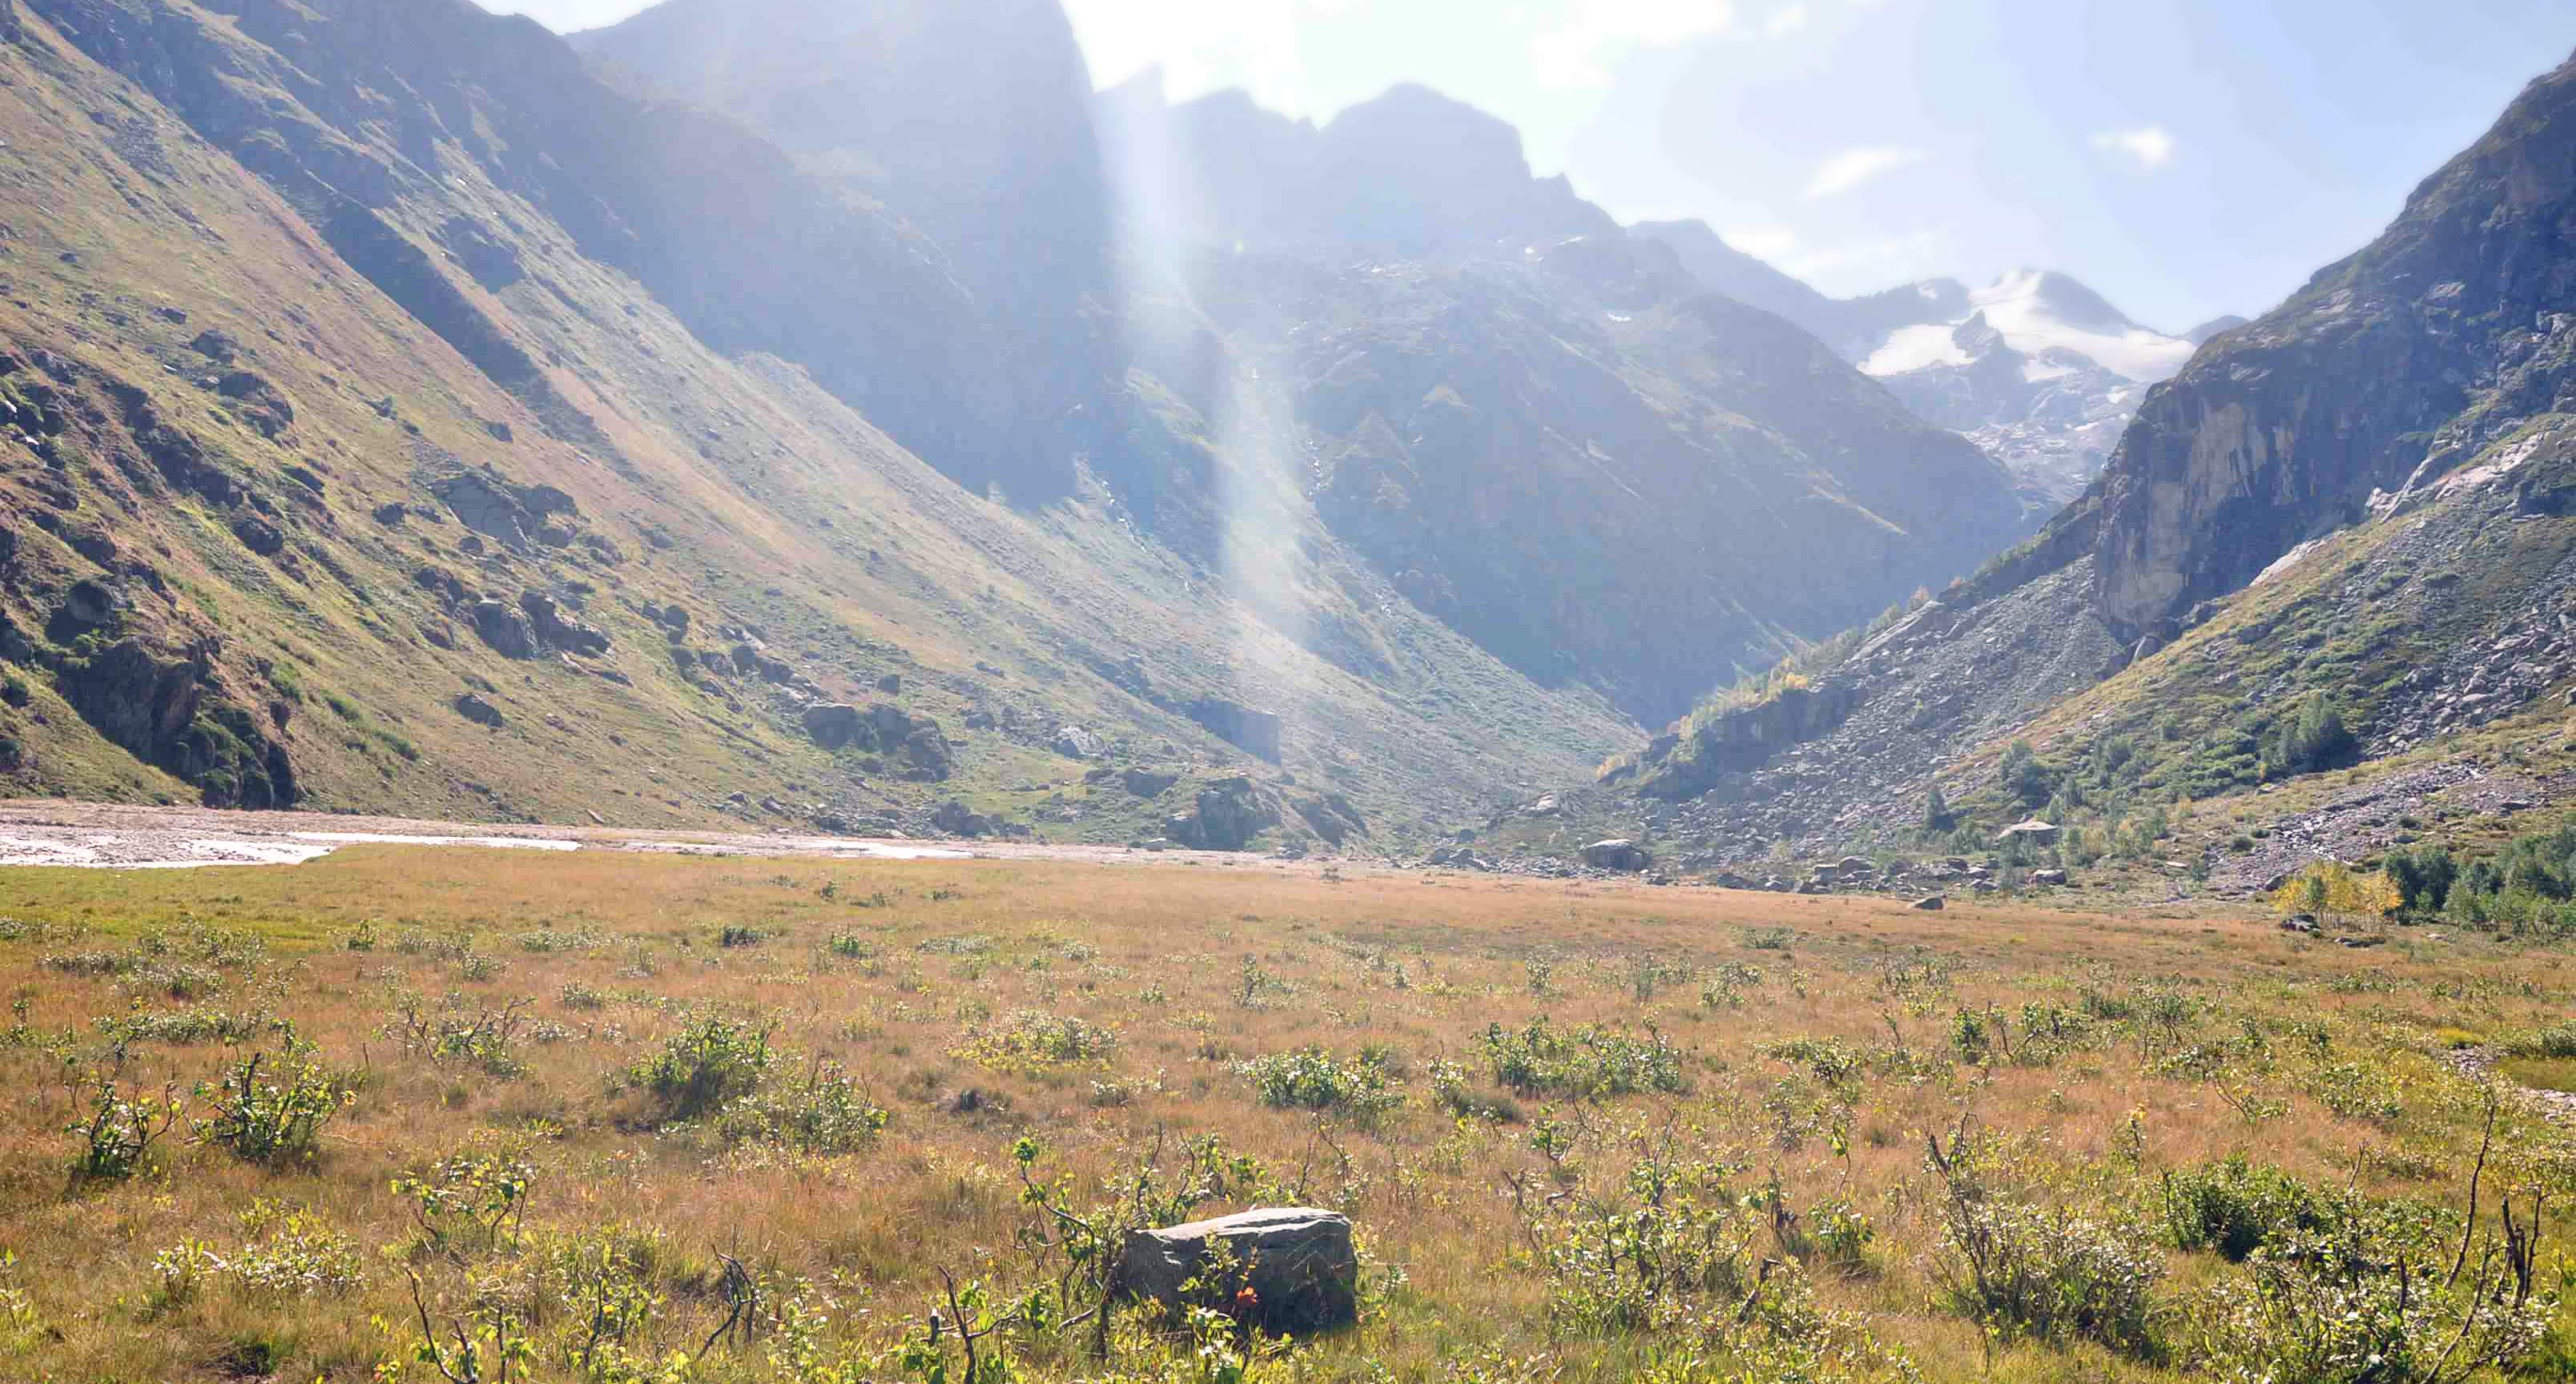
\includegraphics[width=0.7\linewidth]{../pics/DSC_0434 2.jpg}
	\caption{<<Танышханский аэродром>>~--- разлив реки. Наше м.н.}
	\label{fig:DSC_0434}
\end{figure}

В 9:45 выдвинулись вдоль левого берега реки Танышхан вниз по течению по набитой тропе. Тропинка пролегала через россыпи курумника, заросли берёз, вечнозелёных деревьев  и рододендронов~--- идущая впереди часть группы легко терялась из виду. На участке с курумником группа на некоторое время потеряла тропу и шла по курумнику, однако позже выяснилось, что тропа, идущая по низу, в обход курумника, существует, и можно пройти по ней. 

Пройдя ещё немного \alert{(сколько примерно?..)}, мы начали встречать туристов, идущих по правому берегу Танышхана налегке за ягодами. За 400 м до слияния с р. Чунгур-Джар прошли мимо добротного новопостроенного деревянного домика с небольшим хозяйством. К домику подходит автомобильная грунтовка, идущая по правому берегу Танышхана. От неё к домику перекинут хороший металлический автомобильный мост, по которому мы и перешли на противоположный берег. Координаты моста: N 43.27056\degree, E 42.26168\degree. 
 
\begin{figure}[h!]
	\centering
	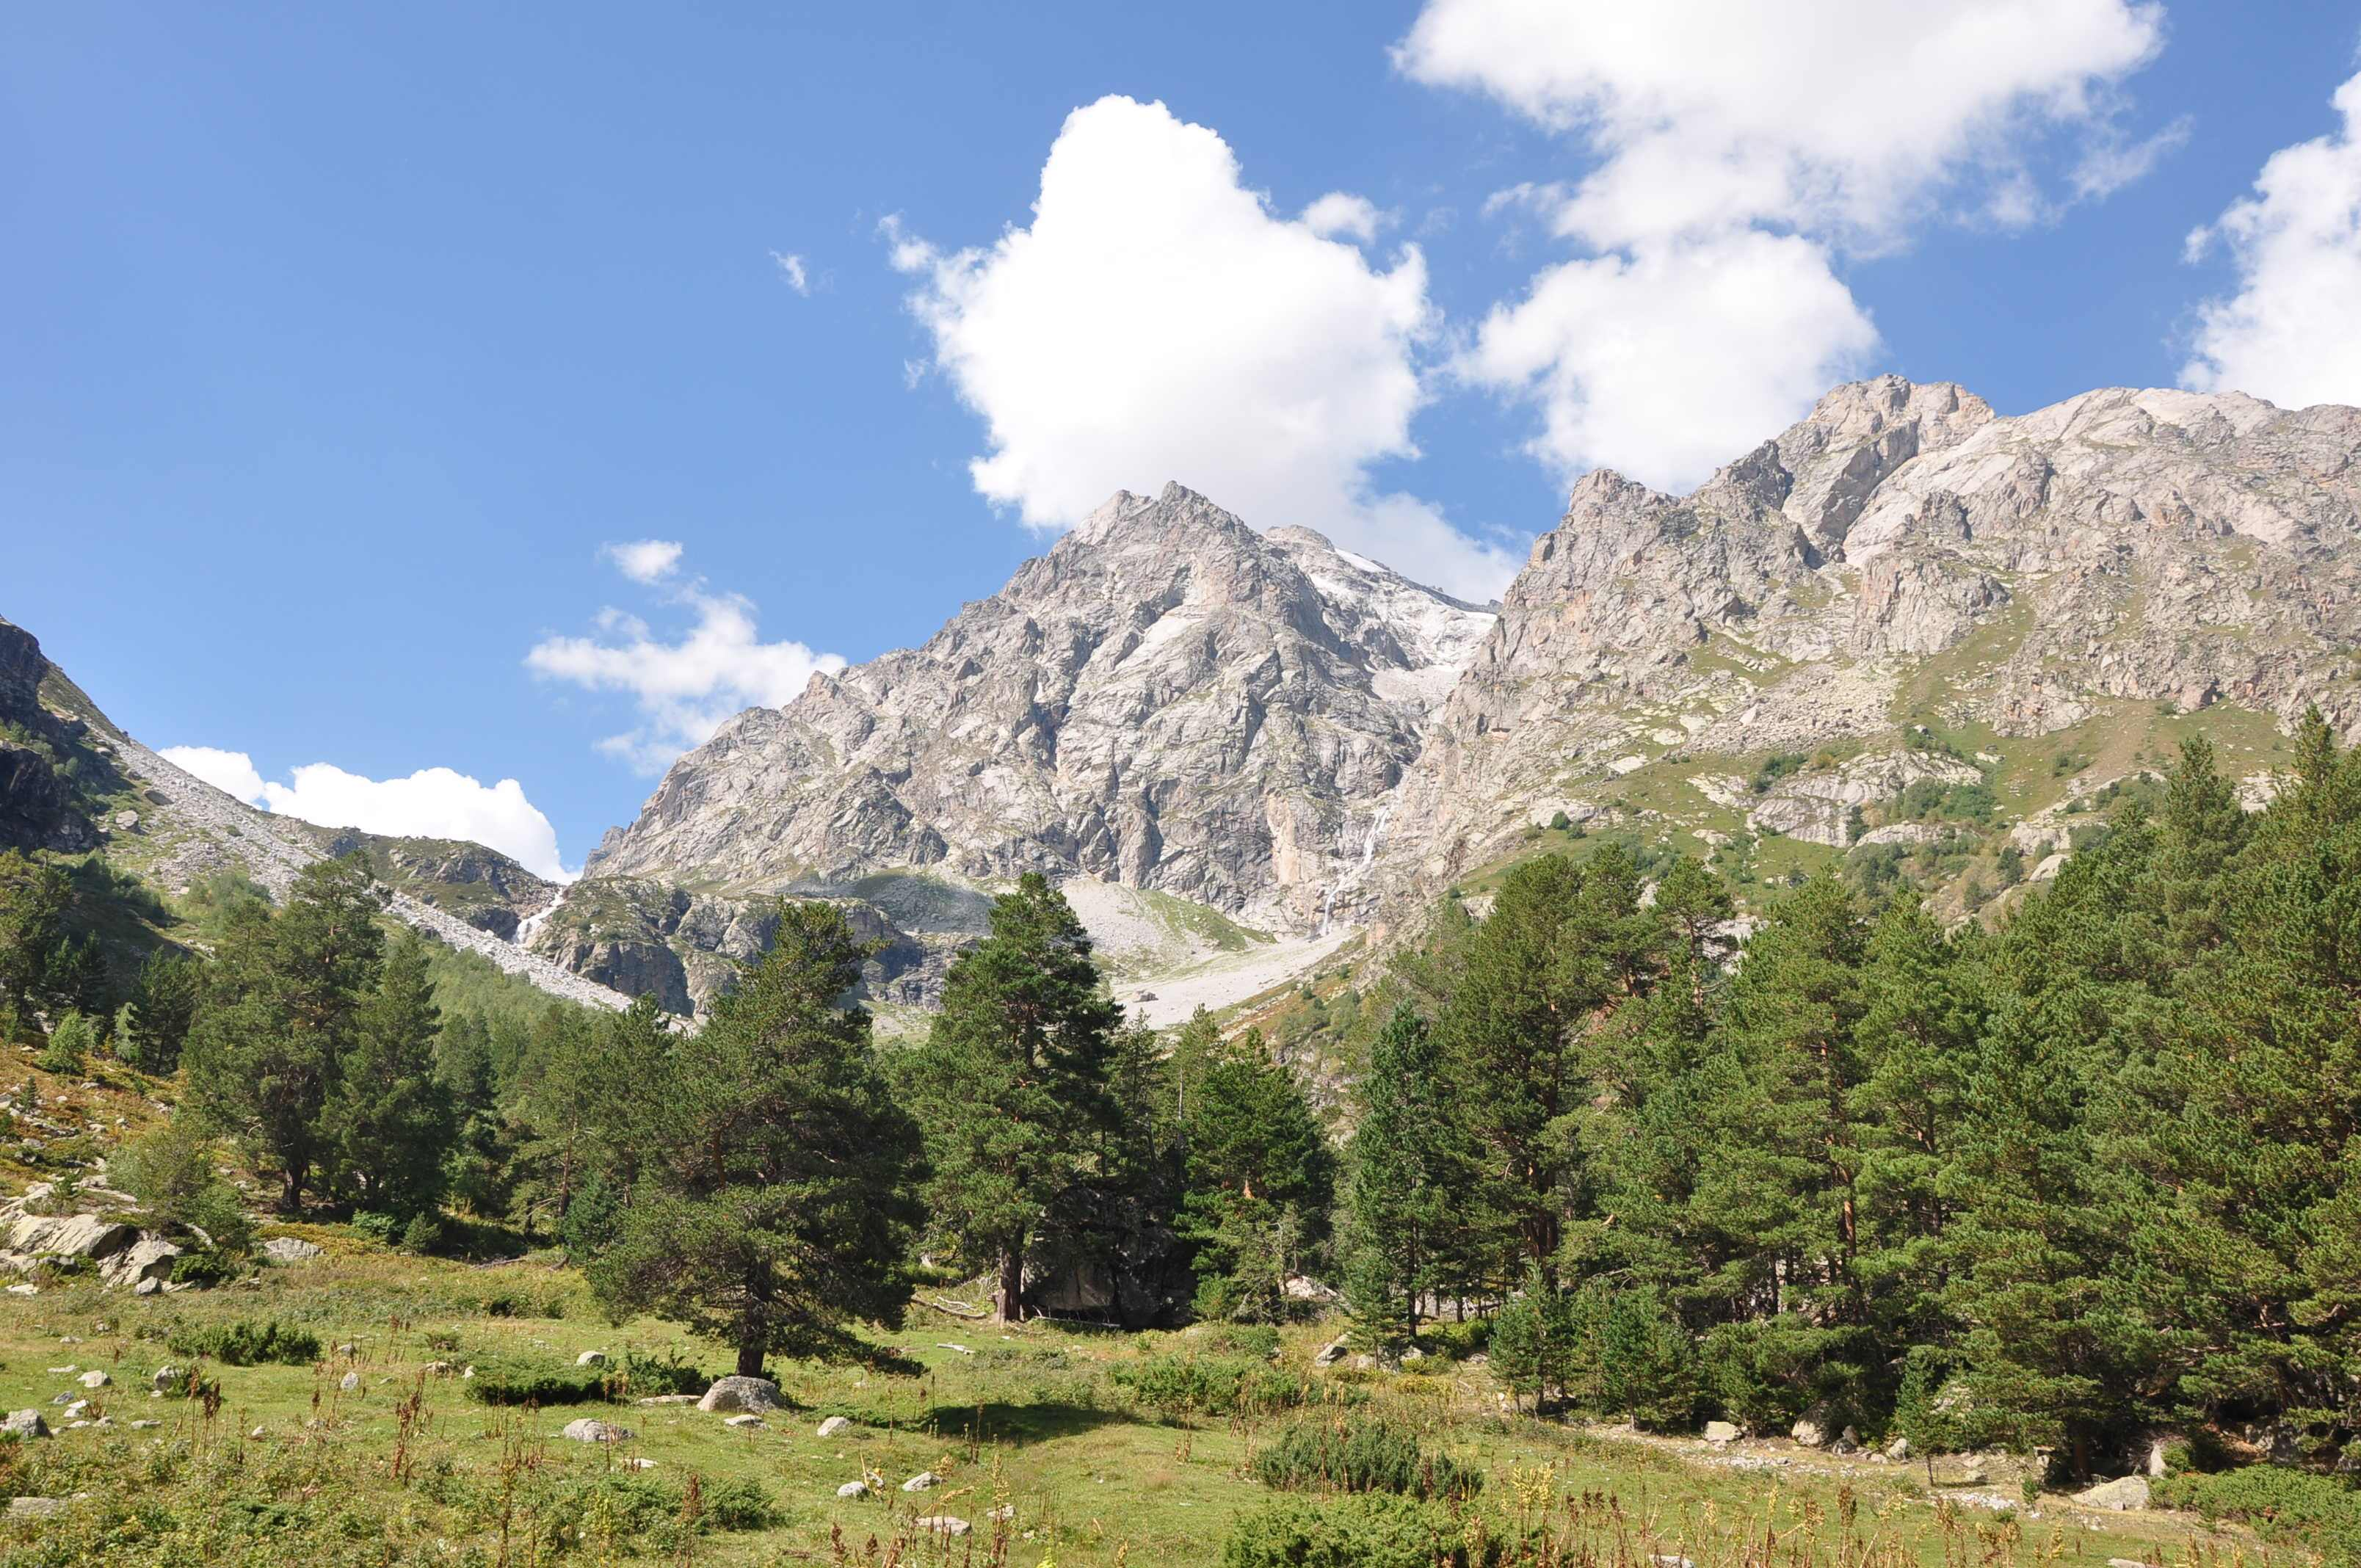
\includegraphics[width=0.7\linewidth]{../pics/DSC_0459 2}
	\caption{Д.р. Чунгур-Джар. Именно эти ступени мы обходили через пер. Перемётный}
	\label{fig:DSC_0459}
\end{figure}

Река, образующаяся от слияния Танышхана и Чунгур-Джара, называется Чиринкол. На правом берегу в 11:10 подошли к летовкам пастухов. Встретили и людей, и непослушное стадо коров. Летовок здесь находится две, на некотором расстоянии друг от друга, и в первой из них хозяйка предложила нам хычины. 

На привале у первой летовки обсудили процедуру схода. Учитывая, что почти половина оставшейся на тот момент группы приняла решение сходить, рассматривался в том числе и тот вариант, при котором завершить поход придётся всей группе. Однако одна из участниц, Даша Казаринова, выразила явное желание продолжать маршрут, --- и, поскольку стало понятно, что сопровождать всю группу на выход не нужно, руководитель однозначно принял решение дойти до конца маршрута с теми, кто останется.

Что касается второй летовки, то вблизи неё должен был быть мост через Чиринкол на левый берег, но поскольку поначалу мы его не заметили, а по правому берегу продолжала идти хорошая грунтовая дорога, мы решили довериться ей и не переходить \alert{(что говорил навигатор: что дорога есть и на правом, и на левом берегу?)}. (В 2018 г. \cite{Korolyov2018} долина Чиринкола была затоплена; по воспоминаниям руководителя, как минимум, в его верховьях ни о какой дороге не было и речи, и группа шла по тропе сначала по правому берегу, а затем по левому.) Что касается нашей группы, то решение идти по правому берегу оказалось ошибочным: в 11:25 группа подошла к автомобильному броду, который сам по себе был довольно глубоким, плюс после которого дорога почему-то терялась. Поэтому мы вернулись назад \alert{(на сколько метров?)} к летовке и спросили у пастухов дорогу. На левый берег Чиринкола действительно был прокинут бревенчатый мост (N 43.2798\degree,~E 42.25481\degree) --- мы перешли по нему и двинулись дальше по пешеходной тропе \alert{(Там была сначала тропа, а потом дорога, --- или сразу дорога?)}. 

В том месте, где был прокинут мост, р. Чиринкол идёт разливами; это заболоченный участок, заросший березняком, не самый простой с точки зрения ориентирования. Дорога по левому берегу с правого берега не просматривается.

\begin{figure}[h!]
	\centering
	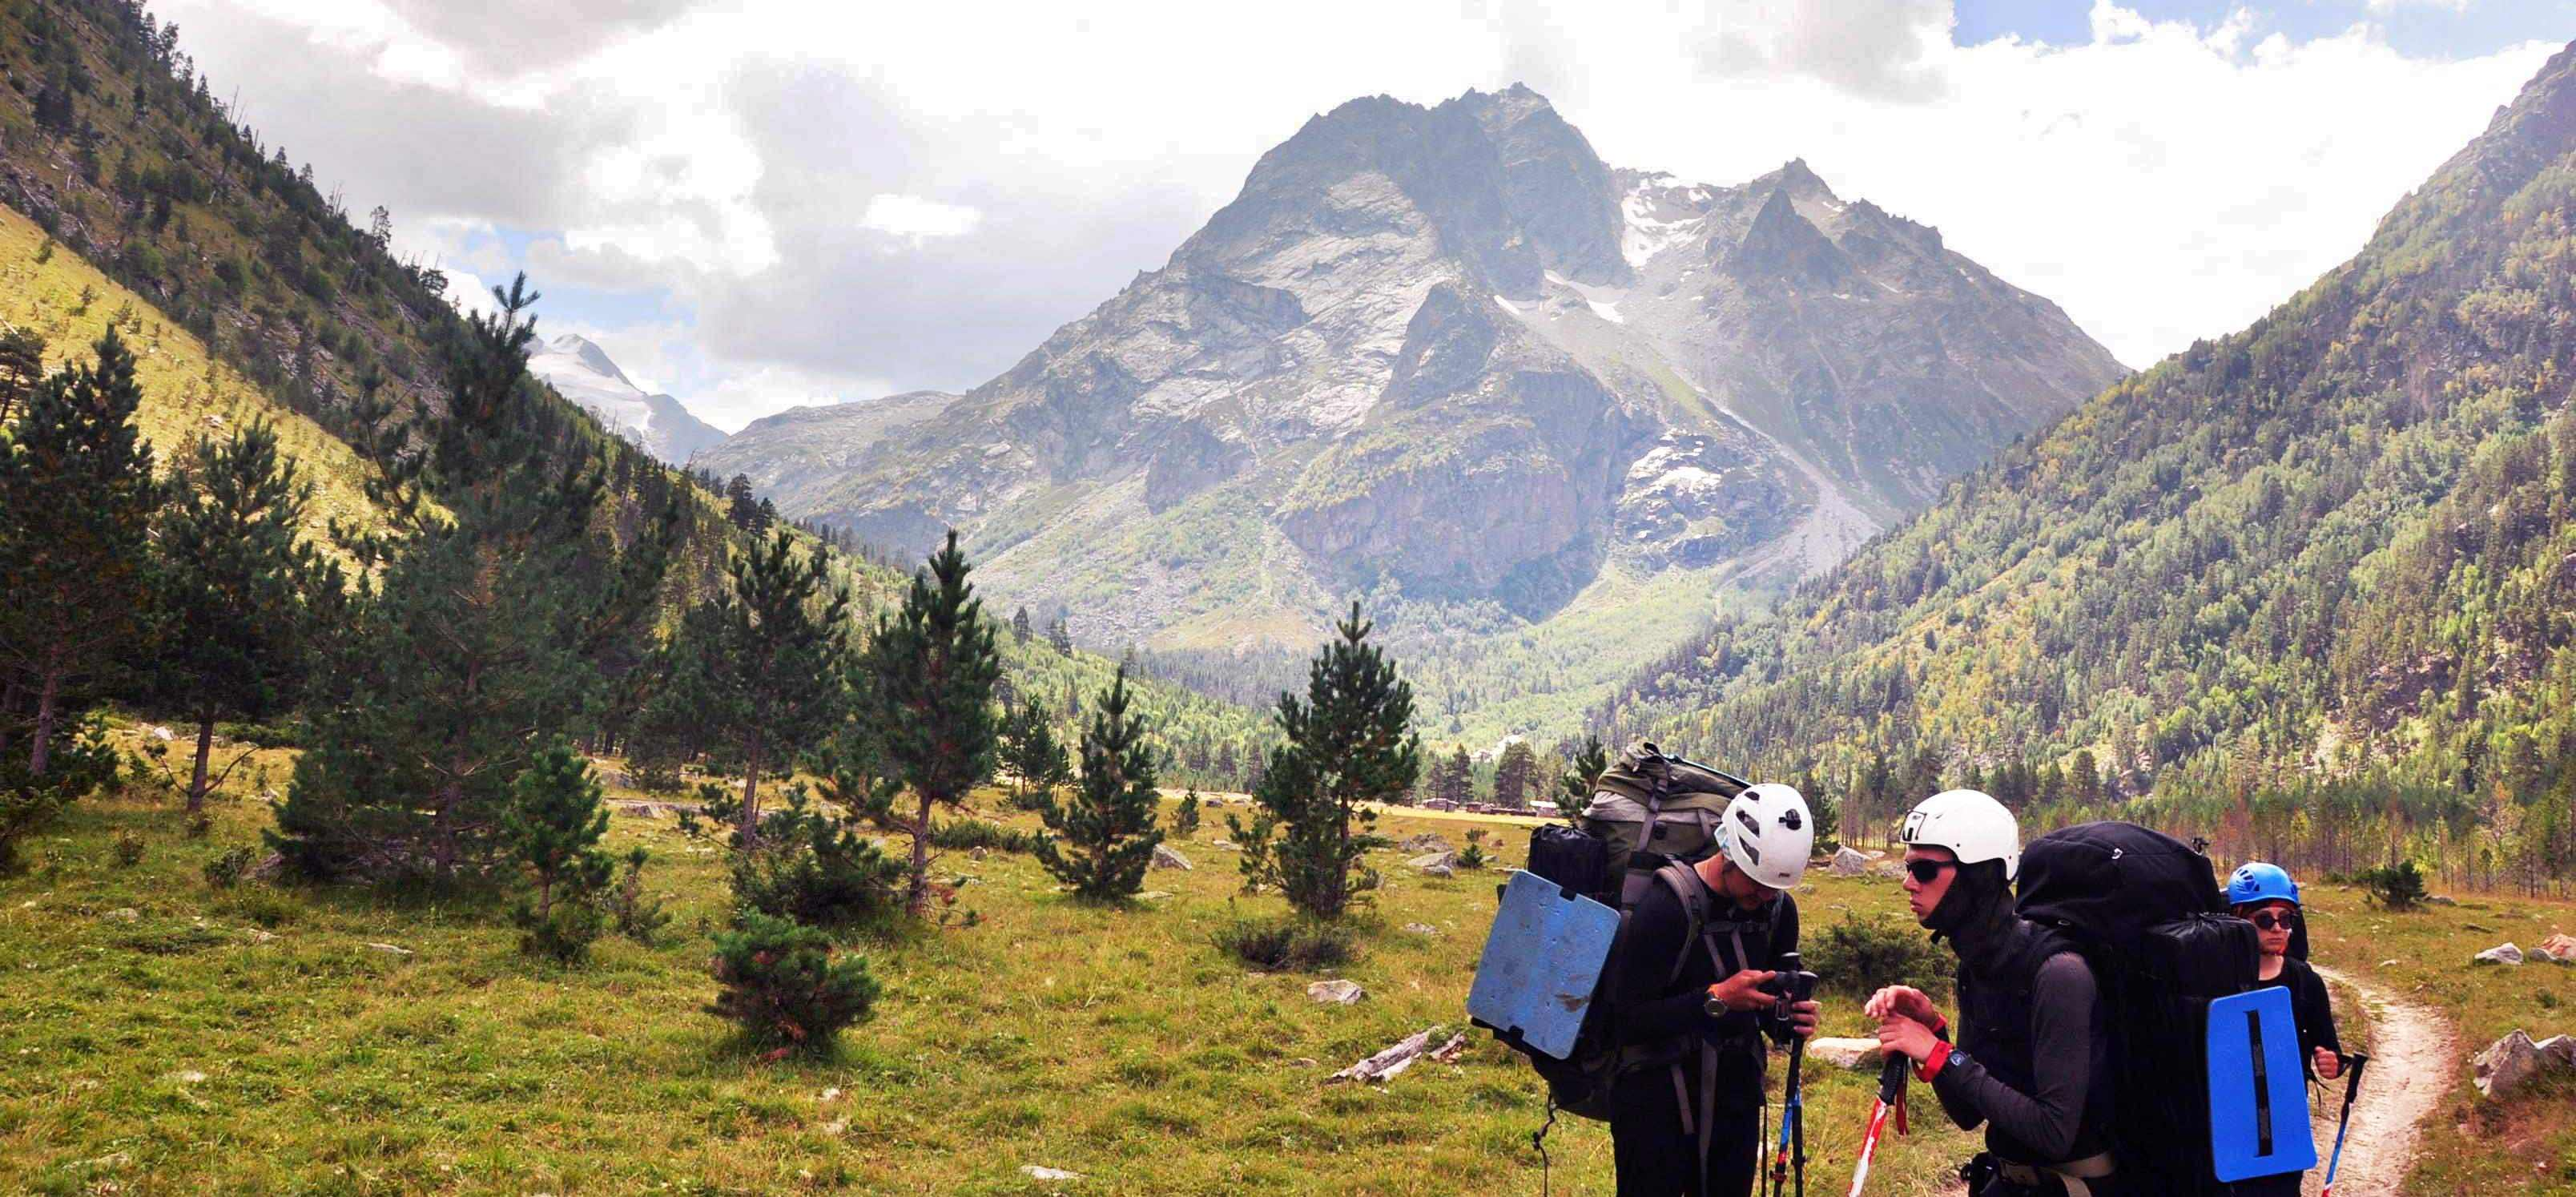
\includegraphics[width=0.7\linewidth]{../pics/DSC_0462 2}
	\caption{Д.р. Чиринкол, вид на слияние р. Танышхан и Чунгур-Джар. Рядом с бродом. На заднем плане виднеется коровник}
	\label{fig:DSC_0462}
\end{figure}

\alert{(С какого-то момента)} группа шла по левому берегу р. Чиринкол по хорошей грунтовой дороге.
 
\begin{figure}[h!]
	\centering
	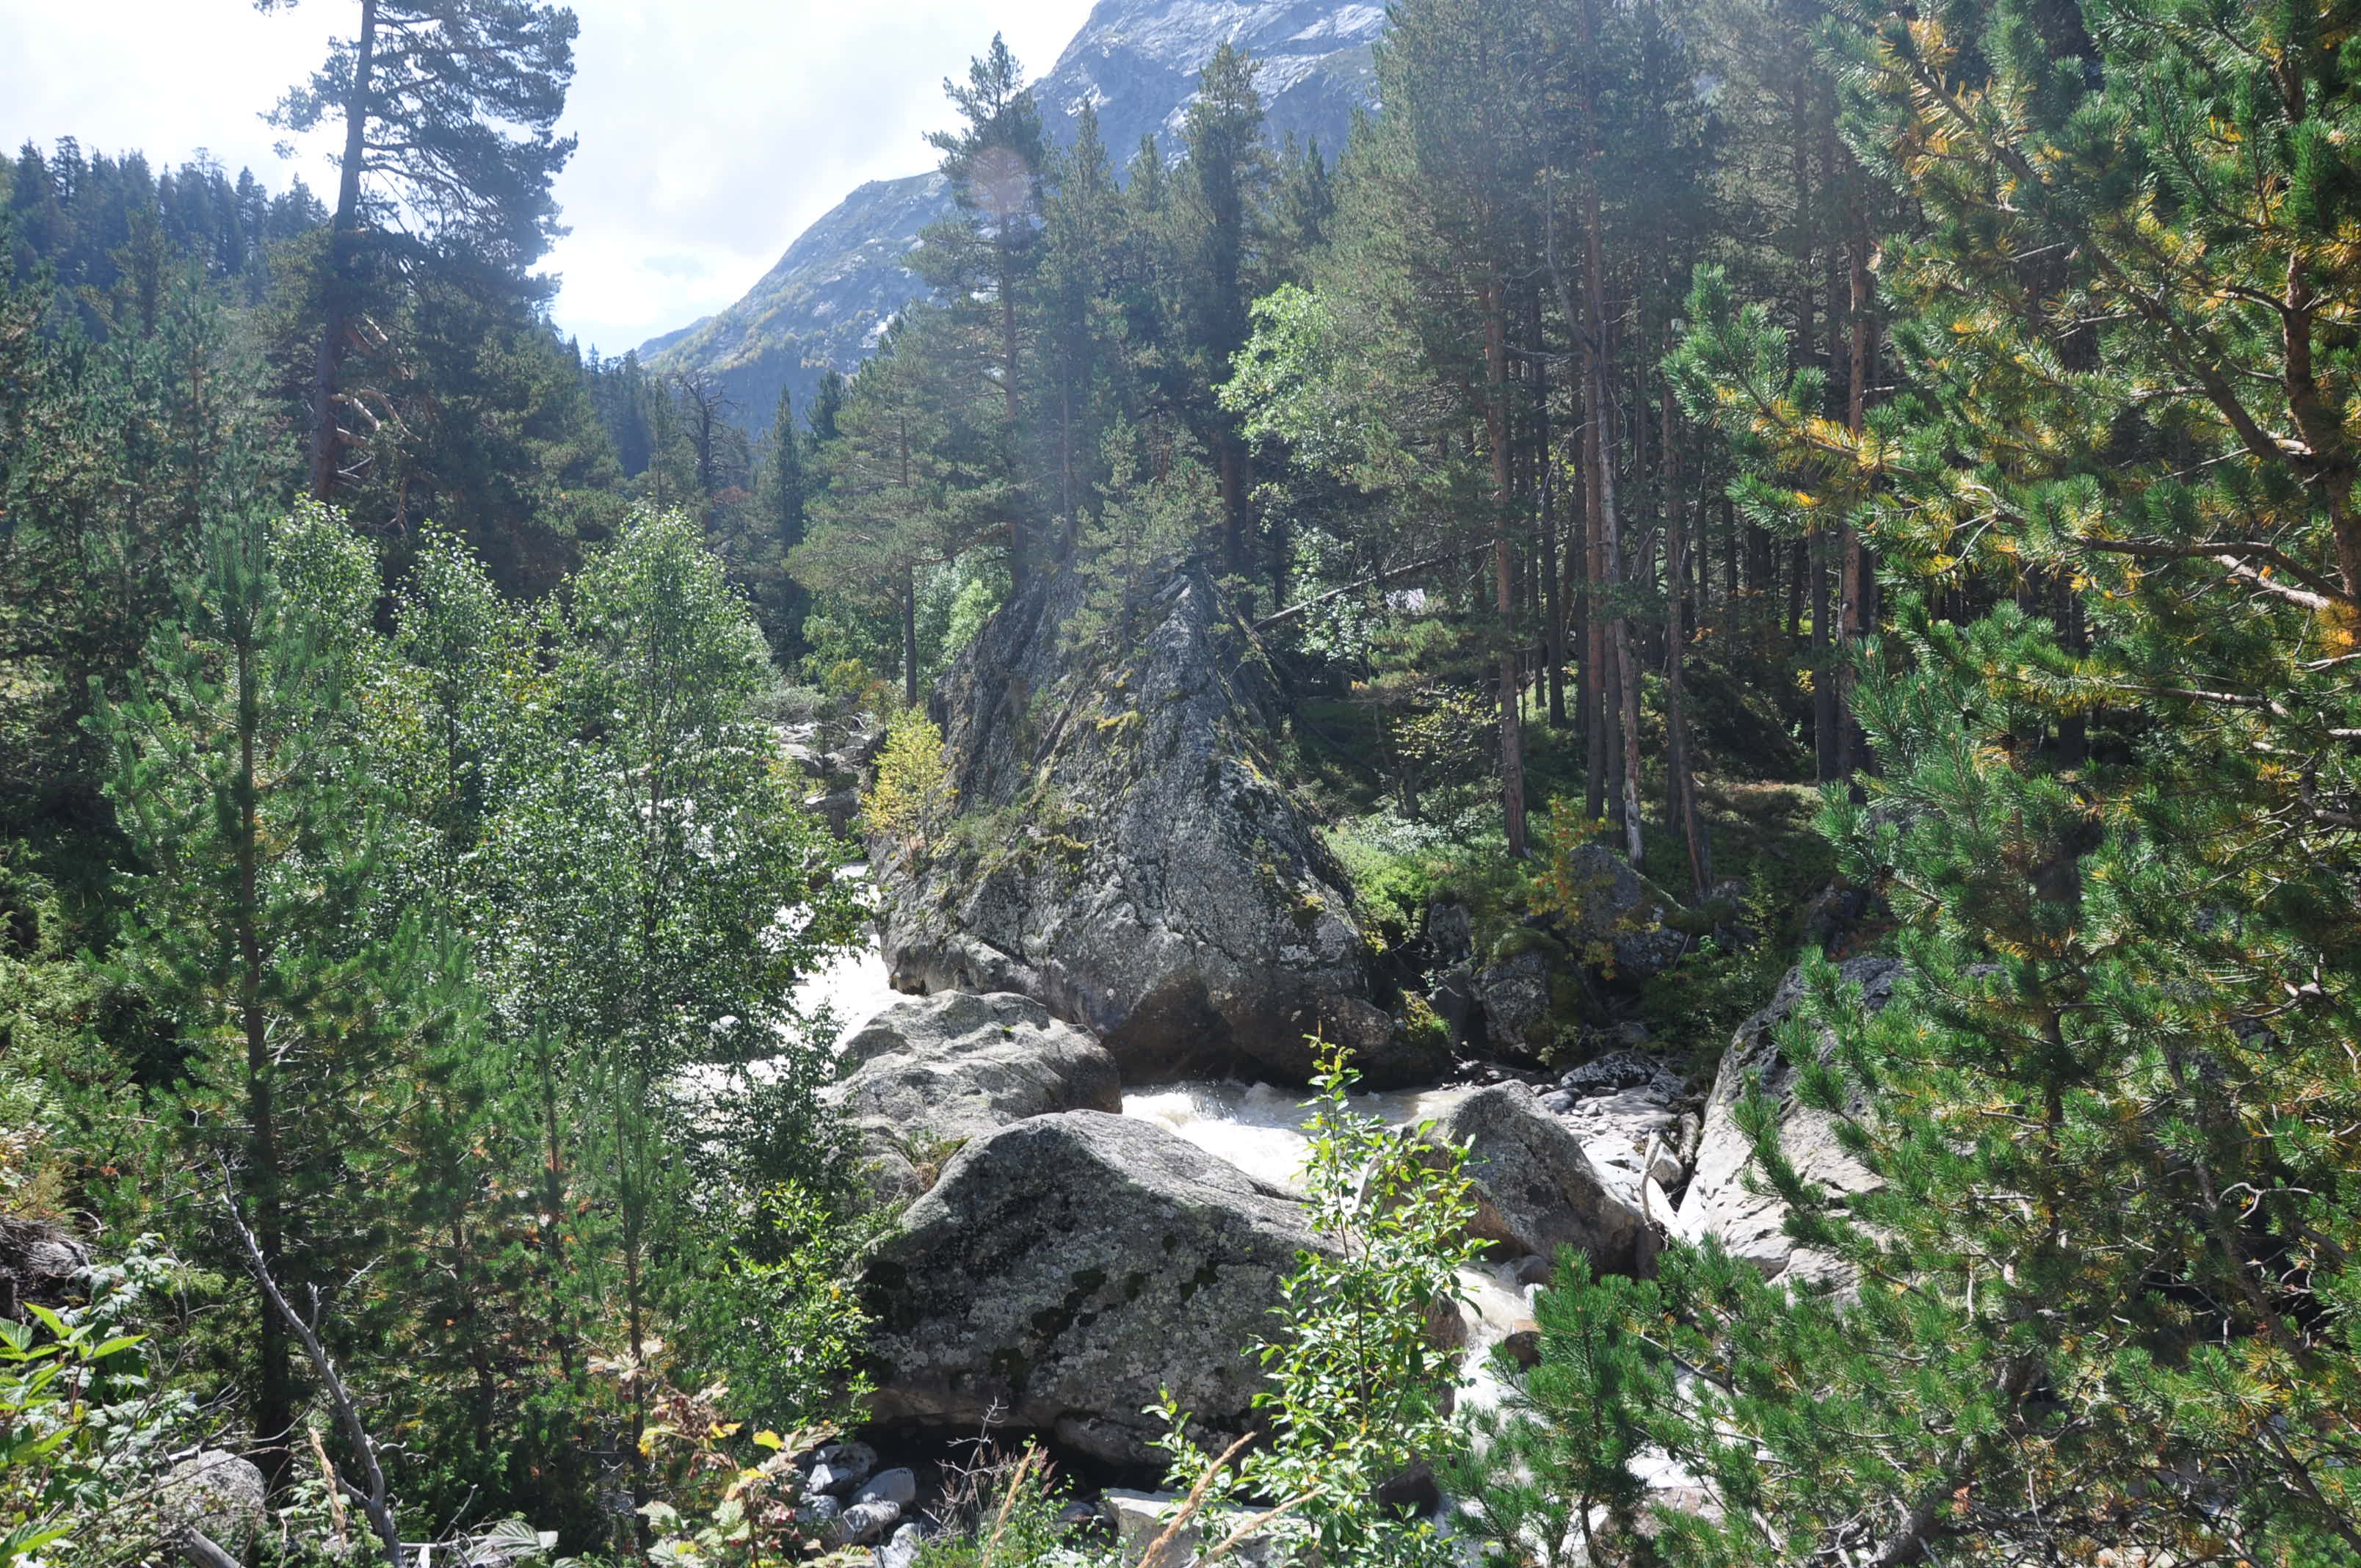
\includegraphics[width=0.7\linewidth]{../pics/DSC_0461 2}
	\caption{р. Чиринкол. Не хотелось бы в неё упасть!}
	\label{fig:DSC_0461}
\end{figure}

Поскольку в этот день прогноз погоды обещал грозу \alert{(Или просто ливень? Чекнуть.)}, и, по воспоминаниям руководителя, выход из висячей долины Чиринкола в д.~р. Кубань был достаточно неприятным, мы торопились выйти к Кубани как можно раньше. Однако в какой-то момент стало понятно, что состояние группы стало совсем неважным, и участникам требуется хотя бы горячий обед. Руководитель распорядился остановиться в ближайшем удобном месте, и в 14:14 группа встала на удобной полянке (N 43.32065° E 42.24355°), не дойдя до слияния рек \alert{сколько км?}. \alert{(Во сколько?)} дошли до слияния и моста через р. Кубань, и в 17:15 встали лагерем на живописном холме в 80 м к востоку от моста через реку (N 43.33085° E 42.24742°). При выходе на дорогу, которая ведёт в верховья Кубани, надо сделать небольшой крюк, вследствие чего фактически от моста нужно пройти \alert{сколько?} км.  Где-то между мостом через Кубань и местом ночёвки группа Королёва ловила сеть \cite{Korolyov2018}, но у нас не получилось. 

Через координатора удалось вызвать трансфер на 11 часов следующего дня от погранзаставы \alert{(как она называлась?)}, поэтому был разработан план, по которому руководитель и замруководителя на следующий день сопровождают сходящих участников до погранзаставы, а затем возвращаются к оставшимся участникам, которые в это время готовят завтрак и собирают рюкзаки, --- и группа идёт под пер. Хотютау. Уточнили количество мест и стоимость машины; руководитель провёл личный опрос; участники перепаковали рюкзаки и стали готовиться ко сну. Психологическое состояние группы стало приходить в норму.

\clearpage